\date{\vspace*{-0.2in}}

%%%\renewcommand{\baselinestretch}{2}
\documentclass[10pt]{sigplanconf}
\nocaptionrule


\newcommand{\footnotenonumber}[1]{{\def\thempfn{}\footnotetext{\small #1}}}
\usepackage[normalem]{ulem}
\usepackage{graphicx}
\usepackage{times}
\usepackage{subfigure}
\usepackage{url}
\urlstyle{rm}

\usepackage{color}
\usepackage{listings}
\usepackage{amsmath}
\usepackage{amsfonts}
\usepackage{amssymb}
\usepackage{comment} 

\newtheorem{thm}{Theorem}
\newtheorem{prop}[thm]{Proposition}
\newtheorem{cor}[thm]{Corollary}
\newtheorem{lem}[thm]{Lemma}
\newtheorem{defn}[thm]{Definition}

\newcommand{\cfunction}[1]{{\bf \tt #1}}
\newcommand{\malloc}{\cfunction{malloc}}
\newcommand{\realloc}{\cfunction{realloc}}
\newcommand{\free}{\cfunction{free}}
\newcommand{\madvise}{\cfunction{madvise}}
\newcommand{\brk}{\cfunction{brk}}
\newcommand{\sbrk}{\cfunction{sbrk}}
\newcommand{\mmap}{\cfunction{mmap}}
\newcommand{\munmap}{\cfunction{munmap}}
\newcommand{\mprotect}{\cfunction{mprotect}}
\newcommand{\mlock}{\cfunction{mlock}}

\hyphenation{app-li-ca-tion}
\hyphenation{Die-Hard}
\hyphenation{Archi-pe-la-go}
\hyphenation{buf-fer}

\lstset{language=c++, basicstyle=\small\ttfamily,frame=single,tabsize=4}

\definecolor{Gray}{cmyk}{0,0,0,0.5}

\begin{document}

%\renewcommand{\baselinestretch}{2}

\conferenceinfo{XXXXXXXXXXXXXXXXXXX}

\title{Sheriff: Detecting and Eliminating False Sharing}

\authorinfo{}

\maketitle
ddafdsf
aadfaf
a
fdaf

afd
afad
faf


adad

afadf

adcfad
\begin{figure*}[!t]
\centering
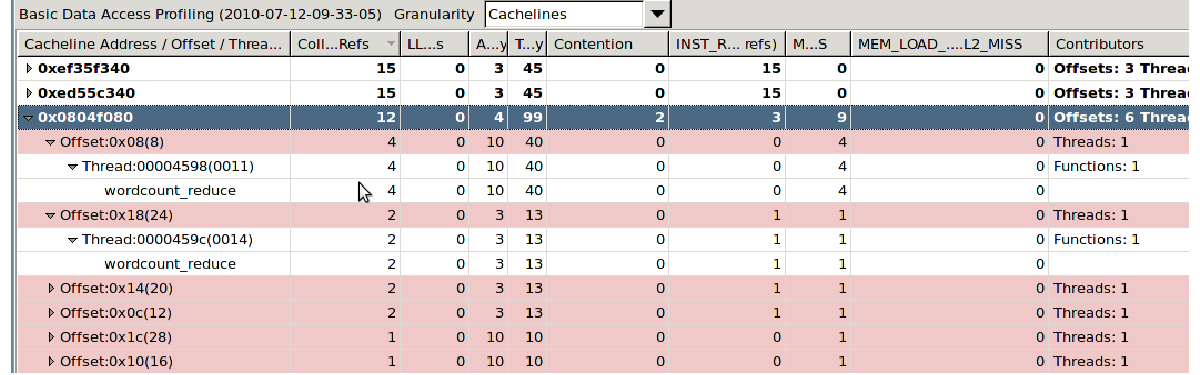
\includegraphics[width=6in]{wordcount.pdf}
\caption{Overview mechanism of Sheriff. }
\end{figure*}

aaa



bbb


ccc


ddd


dddd


eeeee


ffff


ffff


ggg


qqqq

\end{document}
